
\section{\acl{GUI}}
\label{sec:GUI}

\begin{figure}[H]
	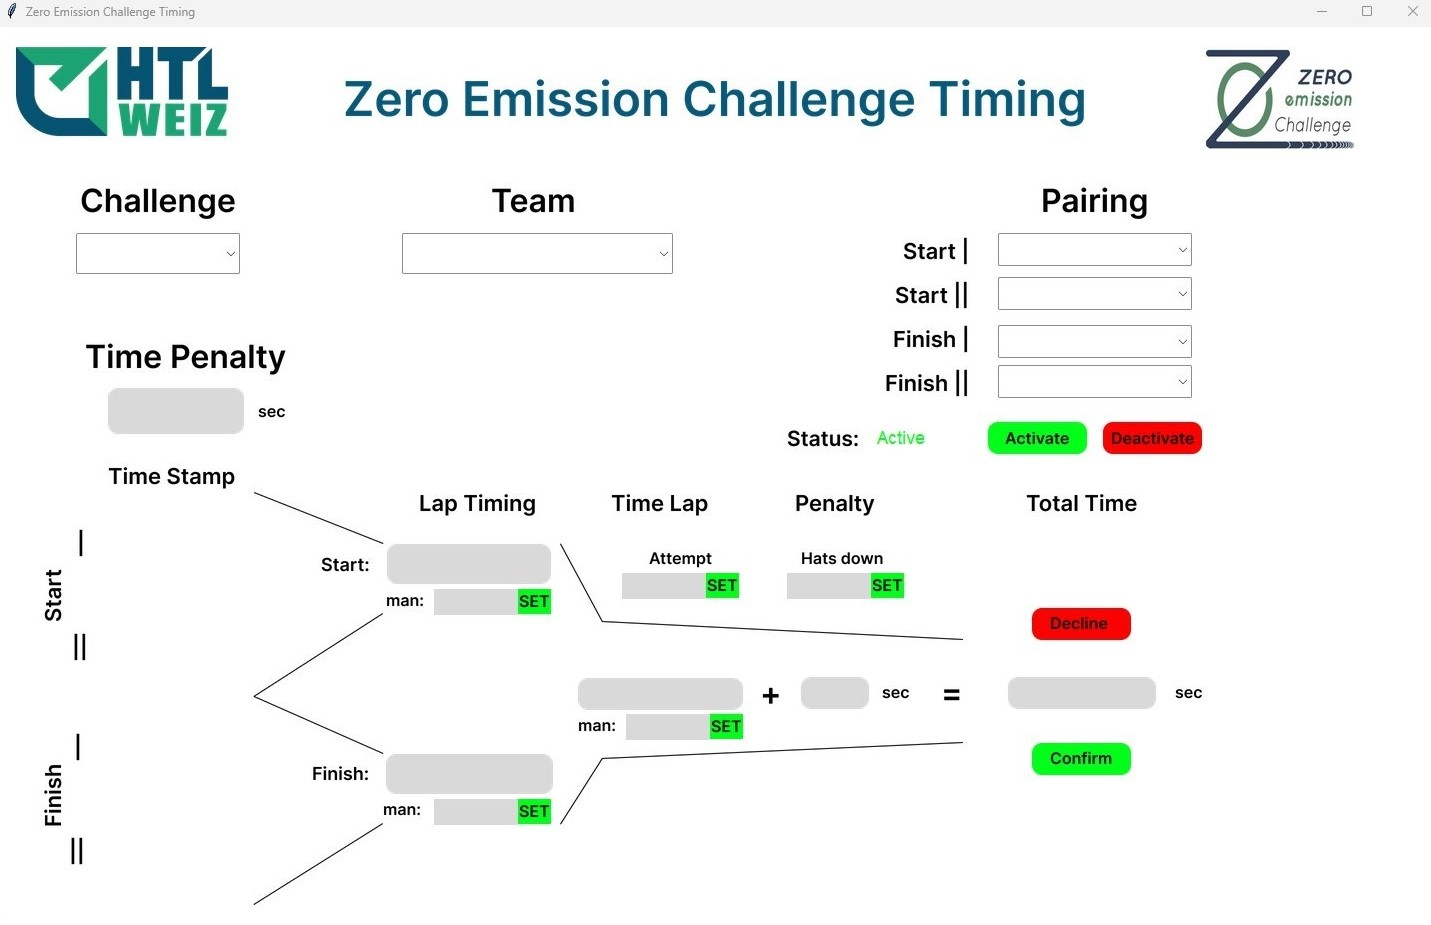
\includegraphics[width=\textwidth]{./01_Inhalte/13_GUI.jpg}
	\centering
	\caption{\ac{GUI}}
	\label{fig:GUI}
\end{figure}

Für die einfache Bedienung dieses Systems wurde eigens eine \ac{GUI} designend. Wie in Abbildung \ref{fig:GUI} zu sehen ist, kann man in der graphischen Benutzeroberfläche die aktuelle Challenge und Team, welche aus der \ac{DB} abgefragt werden, auswählen. Zudem können die verwendeten ESP32 für Start und Ziel ausgewählt werden. Auf der Bedienoberfläche werden von den ausgewählten ESP32 jeweils die letzten vier Zeitstempel angezeigt. Bei Auswahl von zwei Zeitstempeln für den Start bzw. des Ziel (Start | \& Start || oder Finish| \& Finish||), wird der Mittelwert der beiden Zeitstempel berechnet und für die Berechnung der Rundenzeit verwendet. Zudem kann der Start- oder Zielzeitstempel manuell im Format \textbf{hh:mm:ss.ssssss} eingeben und mit dem SET-Button gesetzt werden. Aus dem Start- sowie Finish-Zeitstempel wird die Rundenzeit berechnet, welche auch manuell im Format \textbf{s.ssssss} eingegeben und ebenfalls mit dem SET-Button gesetzt werden kann. Des Weiteren muss noch die Versuchsnummer (Attempt) als \textbf{Ganzzahl} und die umgefahrenen Hüttchen (Hats down) eingegeben werden. Die Zeitstrafe (Penalty) wird durch Multiplikation der \textbf{Hats down} mit dem \textbf{Time Penalty}, welcher auch aus der \ac{DB} entnommen wird, berechnet. Bei vollständiger Eingabe aller Felder bzw. Daten kann der \textbf{Confirm-Button} betätigt werden, wodurch der aktuelle Versuch des Teams in die Datenbank gespeichert wird. Bei Betätigung des \textbf{Decline-Buttons} werden bis auf das ausgewählte Team, Challenge und der ESP32 alle eingegeben Daten zurückgesetzt (das betrifft nicht die letzten vier Zeitstempel der ESP32). Abschließend sollte noch der Statusmodus erklärt werden. Dieser bietet die Möglichkeit Zeitstempel der ESP32 zu berücksichtigen (in der \ac{GUI} anzuzeigen) oder zu ignorieren.


\subsection{Implementierungsschritte}
Damit man die \ac{GUI} ausführen kann, muss man Python installieren. Wichtig ist hierbei das beim Setup-Vorgang \textbf{''Add python.exe to PATH''} angekreuzt wird, damit dem Betriebssystem mitgeteilt wird wo die Python-Interpreter-Datei (python.exe) zu finden ist. Danach muss man noch die benötigten Bibliotheken installieren. Hierfür muss man ein neues Terminal in VS-Code öffnen und folgenden Befehl ausführen damit die benötigten Pakete installiert werden:

\begin{Textfeld1}
	pip install -r ./02\_GUI/requirements.txt
\end{Textfeld1}

Wobei selbstverständlich hier der richtige, relative Pfad eingesetzt werden muss.
Um die Verbindung zwischen der \ac{GUI} und dem MQTT-Broker sowie dem \ac{DBMS} herzustellen, sind einige Anpassungen im \ac{GUI}-Code erforderlich. Es sind zwei wesentliche Änderungen erforderlich: Zum einen muss die \textbf{IP-Adresse} des Servers angepasst werden, und zum anderen müssen die \textbf{Benutzerdaten} in der Datei \textbf{gui.py}, die sich im Ordner \textbf{02\_GUI} befindet,  modifiziert werden. 

\begin{lstlisting}[language=Python]
	# Server configuration
	SERVER_IP = "IP-Address"       
	
	# MQTT configuration
	MQTT_USER = "mqttclient"       
	MQTT_PASSWORD = "Kennwort1"    
	
	# Database configuration
	DB_USER = "mariadbclient"      
	DB_PASSWORD = "Kennwort1"      
\end{lstlisting}

Wichtig ist zudem, dass der Ordern ''\textbf{assets}'' und die Datei ''\textbf{models.py}'' sich auf der gleichen Ordnern-Ebene wie das \ac{GUI}-Programm ''\textbf{gui.py}'' befindet.



